\likechapter{Введение}
\todo[inline, color=red]{2-3 страницы пока не понятно о чем???}
\chapter{Автоматизация производственного планирования}
\section{Система управления и планирования предприятием}
На сегодняшний день, в условиях серьезной конкуренции очень важно следить за всеми новинками технологического прогресса и своевременно внедрять в структуру производства.
Так организация предприятия напрямую влияет на эффективность производства. Основным направлением организацией предприятием в последнее время относят системы ИСУП, которые позволяют достичь следующих задач: выполнение планов производства, оптимизация производственного процесса, снижение издержек и повышение эффективности производства.

Данные системы начали появляться с развитием компьютерных технологий в начале 80-х годов. Одной из главных причин появления данных систем является нехватка административного, бухгалтерского и технического персонала, который обладал бы достаточной квалификацией для обработки информации предприятия, также стало понятно, что предприятия не могут позволять себе большие объемы материального запаса для производства продукции. Это привело к появлению систем планирования потребности в ресурсах. Первым шагом в этом направлении был MRP (Materials Resource Planning), который включал только материалы планирования для производства \cite{MRP}.

Основной концепция MPR заключается в минимизации затрат связанных с запасами, а также расчет сколько и в какие сроки необходимо произвести конечный продукт. 

Недостатками данной системы является, то что при расчете потребностей в материалах не учитываются производственные мощности, их загрузки, трудозатраты и т.д. 

Логическим продолжением MPR системы стала система MPR 2, которая в отличие от предшественника учитывала финансовую составляющую предприятия, а также охватывала более широкий охват ресурсов. Это позволило компаниям иметь более интегрированную бизнес-систему, которая выводила требования к материалам и мощности, связанные с желаемым планом операций, позволяла вводить подробные данные о деятельности, переводить все это в финансовый отчет и предложить план действий для решения тех вопросов, которые были не в соответствии с желаемым планом.

К началу 1990-х годов постоянные улучшения в технологии позволили расширить MRP II, включив в него все планирование ресурсов для всего предприятия. Такие области, как дизайн продукта, хранение информации, планирование мощностей, системы связи, управление персоналом, финансы и управление проектами, теперь могут быть включены в план. Отсюда и термин ERP (Enterprise Resource Planning). И ERP можно использовать не только в производственных компаниях, но и в любой компании, которая хочет повысить конкурентоспособность путем наиболее эффективного использования всех своих активов, включая информацию \cite{ptak_schragenheim_2004} [23,25].

Разрабатываемое программное обеспечение принадлежит к классу ERP-систем. Многие современные ERP-систем разработаны по модульному принципу, поэтому существует возможность выбирать и внедрять только те модули, которые необходимы клиенту. 

В данной работе рассматривается одна из частей ERP систем,отвечающая за сопоставление конструкторских и технологических спецификаций, определяющих состав конечного продукта и ресурсов предприятия. На основании данного сопоставления построение плана производственного процесса, учитывающие ограничения предприятия, а также реализация частных математических моделей. Математические модели призваны оптимизировать производственный процесс в зависимости от специфики предприятия( конвейерное производство ).


\section{Источники роста эффективности}

В промышленности есть огромные неиспользованные резервы роста производительности труда. Они могут быть подразделены на резервы снижения трудоемкости продукции и резервы рабочего времени.( см. рисунок \ref{ris:reserve1})

Резервы снижения трудоемкости выявляются и реализуются в виде экономии рабочего времени, затрачиваемого непосредственно на выполнение рабочих операций.

Резервы фонда рабочего времени реализуются путем повышения эффективности использования рабочего процесса для данного коллектива в течение определенного планового периода\cite{Lenin}. 


\begin{figure}[H]
    \center{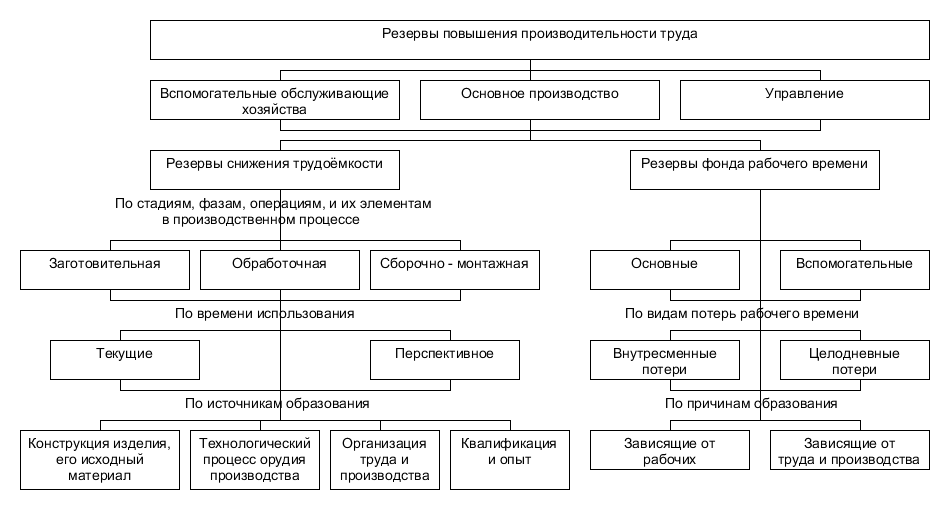
\includegraphics[width=1\linewidth]{fig/reserve1.png}}
    \caption{Резервы роста производительности труда}
    \label{ris:reserve1}
\end{figure}

Исходя из информации представленной на рисунке \ref{ris:reserve1}, можно сделать вывод, что повышение эффективности производства может быть достигнуто, как и грамотной организацией резервов рабочего времени, так и путем пересмотра техники выполнения рабочих операций, но не все резервы повышения производительности можно решить в рамках ИУС. К таким резервам относится конструктивные особенности изделия, так как требуют изменения исходной конструкции продукта, что не является задачей ИУС. 

\section{Обзор методов планирования производственных процессов.}
\subsection{Объемный метод планирования}
\subsection{Календарный метод планирования}
\subsection{Объемно-календарный метод планирования}
\subsection{Объемно-динамический метод планирования}
\section{Постановка задачи}
Цель работы: повышение производительности труда на сборочных производствах за счет автоматизации и оптимизации процессов планирования.

Задачи: 
\begin{enumerate}
    \item Обзор методов и средств повышения производительности труда.
    \item Разработка формальной модели производственных процессов, входных и выходных данных.
    \item Разработка архитектуры подсистемы имитационного моделирования и частных математических моделей.
    \item Разработка алгоритмов имитационного моделирования.
    \item Разработка алгоритмов оптимизации плана работы на такт.
\end{enumerate}